\chapter{伪3D弹幕}

这一章我们将介绍伪3D弹幕相关的数学原理.
伪3D弹幕是通过一些技术手段营造立体感的弹幕, 下图就是一个经典的伪3D弹幕.
实际上子弹本身只能在平面上运动, 它的位置信息总是二维的$x,y$.
伪3D弹幕的整体的制作思路一般是每个子弹由一个三维坐标控制,
通过将三维坐标投影到二维平面来计算子弹的实际坐标.

\begin{center}
  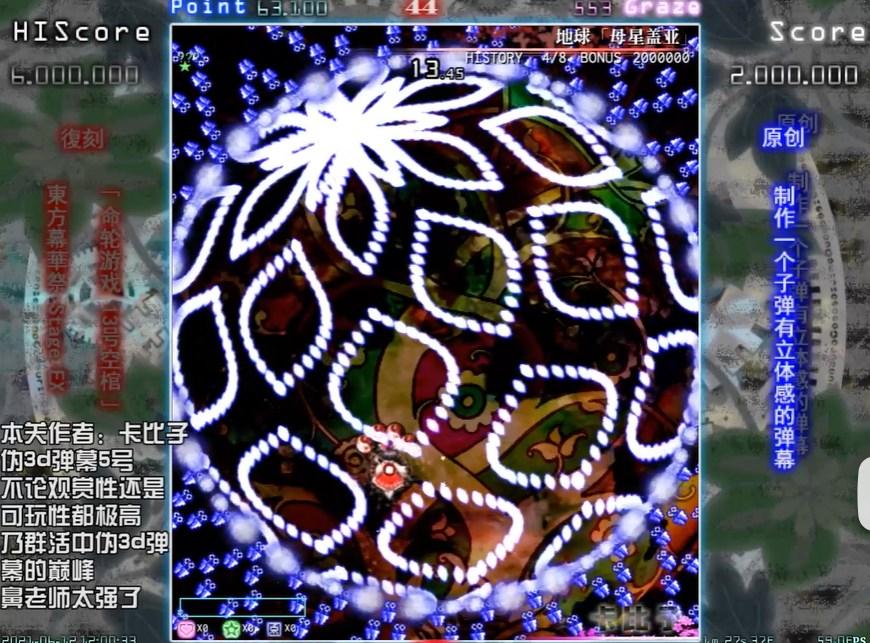
\includegraphics[width=0.6\textwidth]
  {assets/3d/introduction.png}
\end{center}

我们在之前的章节学到的内容大多可以很容易地扩展到三维空间,
这一章会补充一些三维空间相关的内容.
\ref{sec:3d-coord}节将介绍如何用坐标系描述三维空间的位置,
\ref{sec:3d-rotate}节将介绍如何计算三维空间中的旋转,
有了这两节的内容, 结合之前的章节, 我们就可以制作出常规的伪3D弹幕.
额外地, 虽然伪3D弹幕不是必须使用透视投影,
\ref{sec:3d-transform}节将介绍透视投影的原理与计算方法.

\section{三维坐标系与向量} \label{sec:3d-coord}

与二维平面类似, 在三维空间中我们通常使用直角坐标系来表示位置.
三维空间中还有两种比较常见的坐标系: 柱坐标系和球坐标系.

\subsection{空间直角坐标系}

空间直角坐标系是平面直角坐标系在三维空间中的扩展.
如图\ref{fig:xyz-coord},
它由三条两两垂直的坐标轴构成, 三条坐标轴有公共的原点$O$.
将三条坐标轴分别记作$x,y,z$轴, 任取两条坐标轴,
可以确定一个平面, 由此可以确定三个坐标平面,
分别记作$xOy,yOz,zOx$平面.
根据空间中一点$P$在$x,y,z$轴上的对应数值可以确定点$P$的位置,
这也就是点$P$的直角坐标.

\begin{figure}[htbp]
  \centering
  \begin{tikzpicture}[x=(-135:15mm),y=(-15:15mm),z=(90:15mm)]
    \draw[dashed] (0,0,0) -- (1,0,0);
    \draw[-latex] (1,0,0) -- (1.5,0,0) node[left] {$x$};
    \draw[dashed] (0,0,0) -- (0,2,0);
    \draw[-latex] (0,2,0) -- (0,2.5,0) node[right] {$y$};
    \draw[dashed] (0,0,0) -- (0,0,1.5);
    \draw[-latex] (0,0,1.5) -- (0,0,2) node[left] {$z$};
    \node[below] at (0,0,0) {$O$};

    \draw (1,2,0) -- (1,0,0) -- (1,0,1.5) -- (0,0,1.5)
    -- (0,2,1.5) -- (0,2,0) -- (1,2,0)
    -- (1,2,1.5) -- (0,2,1.5) (1,2,1.5) -- (1,0,1.5);

    \node[dot,label={below right,background:
          $P=(1,2,1.5)$}] at (1,2,1.5) {};
    \node[left] at (1,0,0) {1};
    \node[below] at (0,2,0) {2};
    \node[left] at (0,0,1.5) {1.5};
  \end{tikzpicture}
  \caption{空间直角坐标系}
  \label{fig:xyz-coord}
\end{figure}

根据$x,y,z$轴的相对位置,
三维坐标系分为\emph{左手坐标系}和\emph{右手坐标系}两种.
如图\ref{fig:xyz-hand}, 假设在屏幕中有一个空间坐标系,
我们旋转这个坐标系, 使得我们看向屏幕时,
$x$轴水平朝右, $y$轴竖直朝上, 这时$z$轴可能朝向屏幕里面或者外面.
如果$z$轴朝外, 则称之为右手坐标系;
如果$z$轴朝里, 则称之为左手坐标系.

\begin{figure}[htbp]
  \centering
  \begin{subfigure}{0.3\textwidth}
    \centering
    \begin{tikzpicture}[scale=2]
      \begin{scope}[-latex]
        \draw (0,0,0) -- (1,0,0) node[right] {$x$};
        \draw (0,0,0) -- (0,1,0) node[left] {$y$};
        \draw (0,0,0) -- (0,0,1) node[left] {$z$};
      \end{scope}
    \end{tikzpicture}
    \caption{右手坐标系}
  \end{subfigure}
  \begin{subfigure}{0.3\textwidth}
    \centering
    \begin{tikzpicture}[scale=2]
      \begin{scope}[-latex]
        \draw (0,0,0) -- (1,0,0) node[right] {$x$};
        \draw (0,0,0) -- (0,1,0) node[left] {$y$};
        \draw (0,0,0) -- (0,0,-1) node[right] {$z$};
      \end{scope}
    \end{tikzpicture}
    \caption{左手坐标系}
  \end{subfigure}
  \caption{}
  \label{fig:xyz-hand}
\end{figure}

左手坐标系和右手坐标系都有比较广泛的应用.
数学中通常使用右手坐标系,
常见的数学绘图工具比如Desmos, Geogebra都只有右手坐标系可用.
这大概是为了让$x,y$在水平面上, 然后用$z$表示垂直的高度.
而在游戏开发中左手坐标系很常见,
比如LuaSTG的道中背景制作, 使用的就是左手坐标系,
大概是为了让$x$轴向右, $y$轴向上时, 用$z$坐标表示垂直于屏幕向里的深度.

\begin{figure}[htbp]
  \centering
  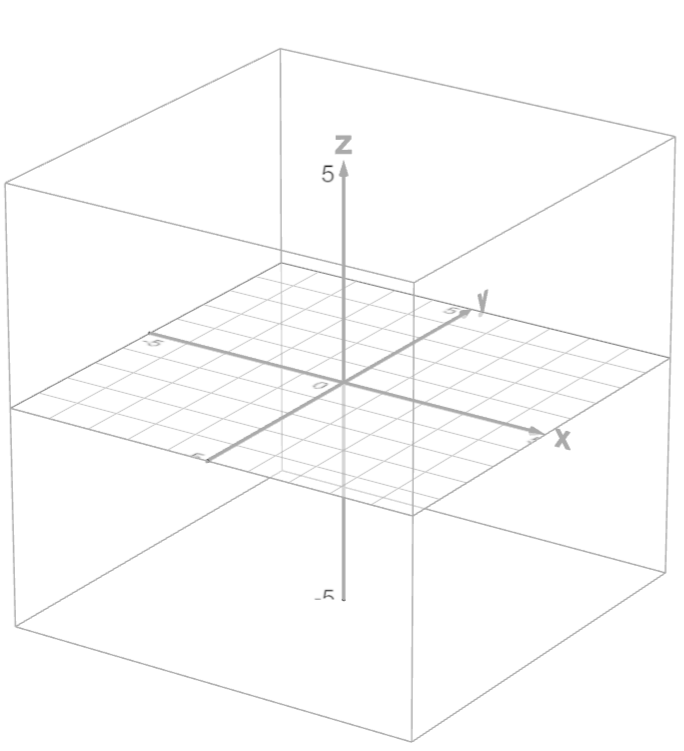
\includegraphics[width=0.3\textwidth]
  {assets/3d/desmos-3d.png}
  \caption{Desmos的3D绘图}
  \label{fig:desmos-3d}
\end{figure}

\subsection{柱坐标系和球坐标系}

如下图所示, 柱坐标系用$xOy$平面上的极坐标$r,\theta$,
以及$z$轴上的坐标$z$确定点的位置.
柱坐标与直角坐标的转换就是$xOy$上的极坐标与直角坐标的转换,
没什么好说的.
\[
  \begin{cases}
    x = r\cos\theta \\
    y = r\sin\theta \\
    z = z
  \end{cases}\quad\quad\quad
  \begin{cases}
    r = \Dist(0,0,x,y)       \\
    \theta = \Angle(0,0,x,y) \\
    z = z
  \end{cases}
\]

\begin{center}
  \begin{tikzpicture}[x=(-135:15mm),y=(-15:15mm),z=(90:15mm)]
    \draw[-latex] (0,0,0) -- (1.5,0,0) node[left] {$x$};
    \draw[-latex] (0,0,0) -- (0,1.5,0) node[right] {$y$};
    \draw[-latex] (0,0,0) -- (0,0,1.5) node[left] {$z$};

    \path (1,0,0) -- (0,0,0) node[above,sloped,midway] {$r$};
    \begin{scope}[canvas is xy plane at z=0]
      \draw (1,0) arc (0:60:1) -- (0,0);
      \draw[->] (2mm,0) arc (0:60:2mm)
      node[midway,below] {$\theta$};
    \end{scope}
    \draw (60:1) -- +(0,0,1.5)
    node[dot,label={right:$(r,\theta,z)$}] {}
    node[midway,right] {$z$};
  \end{tikzpicture}
\end{center}

球坐标系通过球面半径和点在球面上的角来确定点在空间中的位置.
不同资料对球坐标的具体定义有所不同,
本教程采用地理中经纬度的概念来进行定义.
对于空间中的一点$P$, 作一个以原点为球心, 经过点$P$的球面.
设球面的半径为$\rho$, 点$P$在球面上的经度为$\theta$,
纬度为$\phi$ ($-90\degree \le \phi \le 90\degree$).
由$\rho,\theta,\phi$可以确定点$P$的位置.

\begin{center}
  \begin{tikzpicture}[x=(-135:15mm),y=(-15:15mm),z=(90:15mm)]
    \draw[-latex] (0,0,0) -- (1.5,0,0) node[left] {$x$};
    \draw[-latex] (0,0,0) -- (0,1.5,0) node[right] {$y$};
    \draw[-latex] (0,0,0) -- (0,0,1.5) node[left] {$z$};

    \begin{scope}[canvas is xy plane at z=0]
      \draw (1,0) arc (0:75:1) -- (0,0);
      \draw (2mm,0) arc (0:75:2mm)
      node[midway,below] {$\theta$};
    \end{scope}

    \begin{scope}[
        plane x={(75:1)},
        plane y={(0,0,1)},
        canvas is plane,
      ]
      \draw (1,0) arc (0:80:1) coordinate (P);
      \draw (2mm,0) arc (0:80:2mm)
      node[midway,right,background] {$\phi$};
    \end{scope}

    \draw (0,0,0) -- (P) node[dot,label={
          right:$(\rho,\theta,\phi)$}] {};
  \end{tikzpicture}
\end{center}

球坐标$(\rho,\theta,\phi)$与直角坐标$(x,y,z)$有如下转换关系:
\[
  \begin{cases}
    x = \rho\cos\phi \cdot \cos\theta \\
    y = \rho\cos\phi \cdot \sin\theta \\
    z = \rho\sin\phi
  \end{cases}\quad\quad\quad
  \begin{cases}
    \rho = \sqrt{x^2+y^2+z^2} \\
    \theta = \Angle(0,0,x,y)  \\
    \phi = \arcsin\dfrac{z}{\rho}
  \end{cases}
\]

\section{三维向量}

我们在第二章所讲的关于向量的大部分内容可以直接用到三维向量上,
比如向量的几何意义, 线性运算, 线性变换等.
这里我们补充一下三维向量的内积和外积.

三维向量的内积与二维差不多, 向量
$\vec r_1=(x_1,y_1,z_1),\ \vec r_2=(x_2,y_2,z_2)$
的内积为
\[
  \vec r_1 \cdot \vec r_2 = x_1x_2 + y_1y_2 + z_1z_2.
\]

内积的几何意义也差不多, 设$\vec r_1,\vec r_2$的夹角为
$\theta$ ($0\degree \le \theta \le 180\degree$), 则有
\[
  \vec r_1 \cdot \vec r_2 = |\vec r_1|\cdot|\vec r_2| \cos\theta.
\]

两个三维向量的外积是一个新的三维向量.
设三维向量$\vec r_1,\vec r_2$的外积为
$\vec r_3 = \vec r_1\times\vec r_2$,
则有以下性质:

\begin{enumerate}
  \item $\vec r_3$的长度是确定的:
        设$\vec r_1,\vec r_2$的夹角为$\theta$
        ($0\degree \le \theta \le 180\degree$), 则有
        \[
          |\vec r_3| = |\vec r_1|\cdot|\vec r_2|\cdot|\sin\theta|.
        \]
  \item $\vec r_3$的方向是确定的.
        $\vec r_3$垂直于$\vec r_1$和$\vec r_2$ (构成的平面)
        \footnote{
          如果$\vec r_1,\vec r_2$共线,
          那么$\vec r_1\times\vec r_2$的长度为0,
          不用考虑其方向.
        }.
        如下图, 如果使用右手坐标系,
        那么$\vec r_1,\vec r_2,\vec r_3$也构成右手系.
        左手坐标系同理.

        \begin{center}
          \begin{tikzpicture}[
              x=(-135:7mm),y=(0:10mm),z=(90:10mm)
            ]
            \begin{scope}[
                plane x={(1,0,0)},
                plane y={(0,1,0)},
                canvas is plane,
              ]
              \fill[blue!10] (-2.5,-2.5) rectangle (2.5,2.5);
            \end{scope}

            \begin{scope}[-latex]
              \draw (0,0,0) -- (2.5,0,0) node[left] {$x$};
              \draw (0,0,0) -- (0,2.5,0) node[right] {$y$};
              \draw (0,0,0) -- (0,0,2.5) node[left] {$z$};
            \end{scope}

            \coordinate (a) at (1.5,1,0);
            \coordinate (b) at (1,2,0);
            \coordinate (c) at (0,0,1.5);

            \begin{scope}[->]
              \draw (0,0,0) -- (a) node[below] {$\vec r_1$};
              \draw (0,0,0) -- (b) node[below] {$\vec r_2$};
              \draw (0,0,0) -- (c) node[left] {$\vec r_3$};
            \end{scope}
          \end{tikzpicture}
        \end{center}

        特别地, 设$x,y,z$轴的单位向量为$\vec i,\vec j,\vec k$, 则有
        \[
          \vec i\times\vec j = \vec k,\quad
          \vec j\times\vec k = \vec i,\quad
          \vec k\times\vec i = \vec j.
        \]
  \item 反交换律和线性性, 与二维向量的外积相同.
\end{enumerate}

设$\vec r_1=(x_1,y_1,z_1),\vec r_2=(x_2,y_2,z_2)$,
则外积$\vec r_1\times\vec r_2$的计算结果为
\[
  \vec r_1\times\vec r_2 =
  (y_1z_2 - y_2z_1, z_1x_2 - z_2x_1, x_1y_2 - x_2y_1).
\]
三个分量对应三组二维向量的外积, 比如$x$坐标,
是$\vec r_1,\vec r_2$在$yOz$平面上的投影
$(y_1,z_1),(y_2,z_2)$的外积, $y,z$坐标同理.

\section{三维向量与定轴旋转} \label{sec:3d-rotate}

\section{视图变换} \label{sec:3d-transform}

视图变换 (viewing transformation)
是由多个特定变换组合成的一套变换,
其目的是将虚拟空间中的物体变换到屏幕平面上.
视图变换包含四个步骤:
\begin{enumerate}
  \item 模型变换 (modeling transformation):
        将模型空间变换到世界空间, 从而把物体放置到场景中应在的位置.
  \item 摄像机变换 (camera transformation):
        在场景中设置一个摄像机, 将世界空间变换到摄像机空间.
  \item 投影变换 (projection transformation):
        将摄像机空间投影到标准平面, 一般使用
        正交投影 (orthographic projection)
        或透视投影 (perspective projection).
  \item 视口变换 (viewport transformation):
        将标准平面变换到屏幕平面.
\end{enumerate}

我们用两个例子来说明视图变换的流程.
其一是一个伪3D弹幕 (详见视频
\url{https://www.bilibili.com/video/BV1P54y1n7M3/}的18分40秒),
子弹在球面上运动, 球面本身也不断转动.
其二是LuaSTG如何将3D背景的位置变换到屏幕上.

\begin{center}
  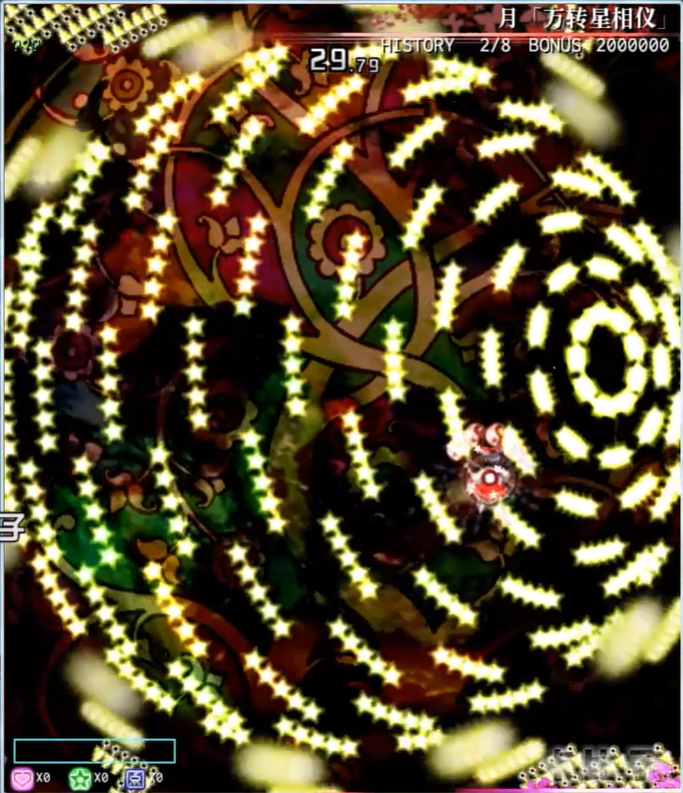
\includegraphics[width=0.3\textwidth]
  {assets/3d/3d-spellcard.png}
  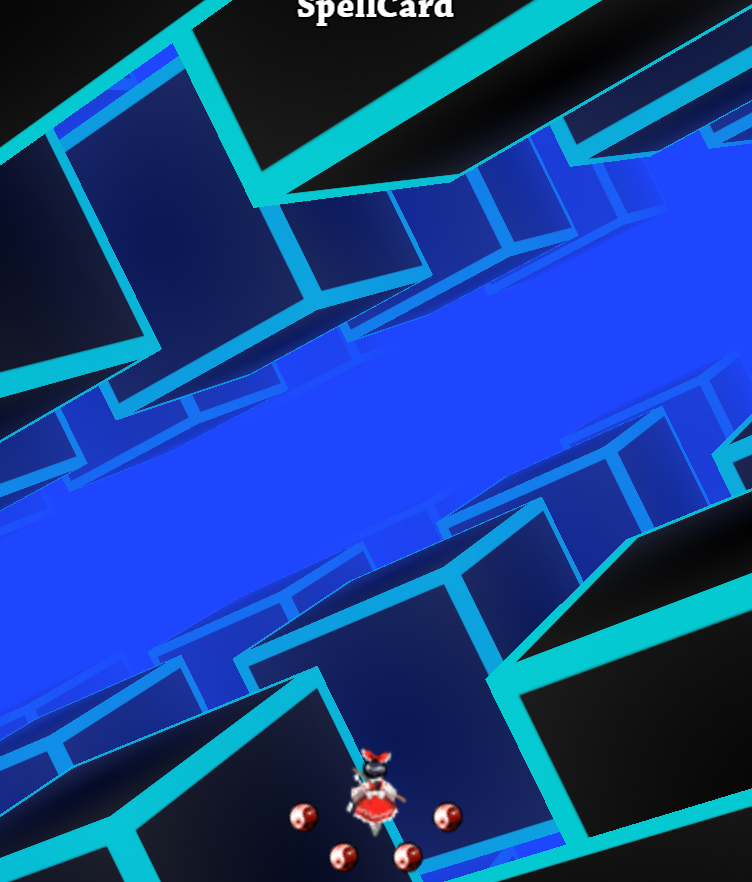
\includegraphics[width=0.3\textwidth]
  {assets/3d/3d-background.png}
\end{center}

\subsection{例1: 伪3D弹幕}

伪3D弹幕主要涉及视图变换的第一步, 将模型空间变换到世界空间.

使用子弹在球面上的球坐标可以方便地描述各个子弹的运动,
我们按照\ref{sec:3d-coord}节球坐标的部分建立直角坐标系,
坐标系的原点为球心, 单位长度为球半径.
这个坐标系对应的就是模型空间.
建立模型空间使得我们可以方便地描述子弹的运动:

首先, 子弹的生成和运动是基于球坐标 (经度和纬度) 的.
假设我们用横坐标代表经度, 纵坐标代表纬度, 那么子弹的生成和运动逻辑大致如下:

\begin{center}
  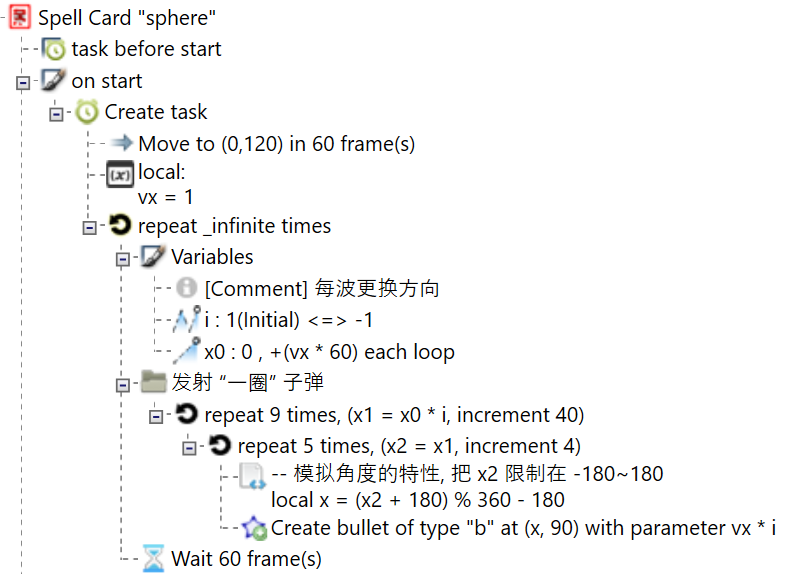
\includegraphics[width=0.49\textwidth]
  {assets/3d/eg1-1.png}
  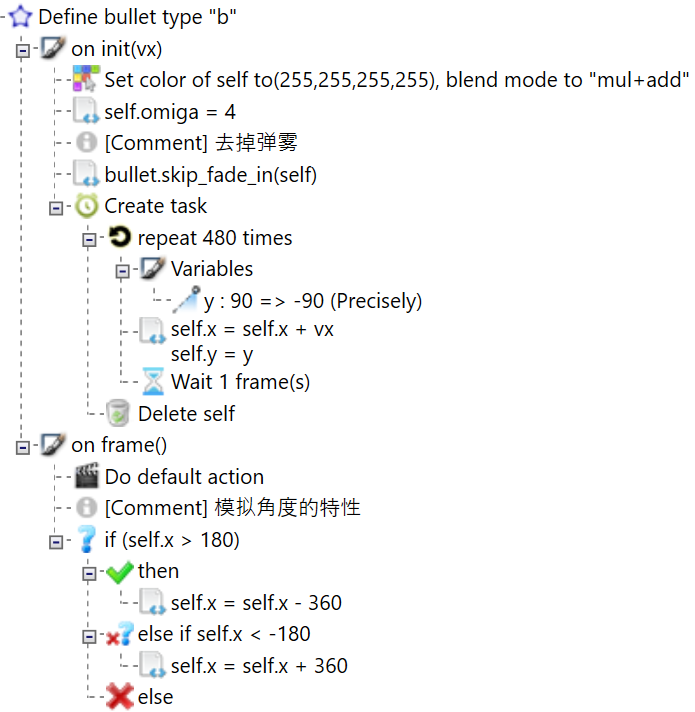
\includegraphics[width=0.49\textwidth]
  {assets/3d/eg1-2.png}
  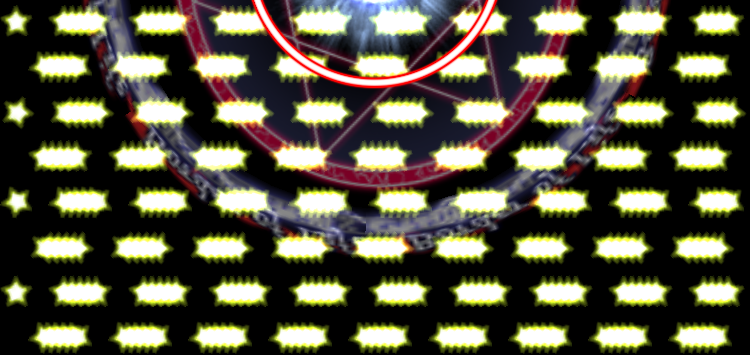
\includegraphics[width=0.6\textwidth]
  {assets/3d/eg1-3.png}
\end{center}

在模型空间中, 子弹所在的球面不会转动, 球面半径为1,
于是从球坐标到直角坐标的转换非常容易.
设子弹在球面上的经度为$\theta$, 纬度为$\phi$,
则子弹在模型空间中的坐标为
\[
  x = \cos\phi\cos\theta,\quad
  y = \cos\phi\sin\theta,\quad
  z = \sin\phi.
\]

模型变换把模型空间中的物体经过平移, 旋转, 缩放等基础变换
放到游戏场景 (世界空间) 中.
我们把世界空间设置为屏幕平面$xOy$加上垂直于屏幕向外的$z$轴,
此时世界空间的$x,y$坐标直接对应子弹的\raw{self.x}, \raw{self.y}属性,
视图变换的后三步就不需要了.
在这个例子中, 我们只需要根据球面的朝向进行旋转,
然后把球面半径从1放大到180 (换言之, 把$x,y$放大到180倍),
即可完成模型变换.

我们可以用空间的基底 (3个三维向量) 来表示球面的朝向.
考虑模型空间的坐标轴向量被变换到哪里:
\begin{itemize}
  \item 在初始时刻,
        模型空间的$x$轴单位向量对应世界空间的$z$轴单位向量$(0,0,1)$,
        类似地, 模型空间的$y,z$轴单位向量分别对应世界空间的
        $(1,0,0), (0,1,0)$,
        所以初始时刻旋转变换对应的基底为
        $((0,0,1),(1,0,0),(0,1,0))$.
  \item 球面的朝向随时间不断旋转,
        在每个瞬时, 球面的旋转可以看作定轴旋转,
        可以用\ref{sec:3d-rotate}节介绍的方法进行计算.
        由于旋转变换是线性的, 我们可以直接对各个基底向量计算旋转, 计算结果作为新的基底,
        从而得到球面的朝向变化.
\end{itemize}

总结一下整个处理流程:
\begin{center}
  \begin{tikzpicture}
    \node[draw] (a) at (0,0) {球坐标};
    \node[draw] (b) at (2.5,0) {模型空间坐标};
    \node[draw] (c) at (7,0) {世界空间坐标};
    \node[draw] (d) at (9.8,0) {子弹属性};
    \draw[->] (a) -- (b);
    \draw[->] (b) -- (c) node[midway,above] {\scriptsize 旋转, 放缩};
    \draw[->] (c) -- (d);
    % \node (e) at (0,-1) {\footnotesize 子弹运动};
    \node (f) at (4.75,-1) {\footnotesize 旋转变换的基底};
    % \draw[->] (e) -- (a);
    \draw[->] (f) -- (4.75,0);
  \end{tikzpicture}
\end{center}

图\ref{fig:3d-spellcard-code}展示了根据上述方法编写的伪3D弹幕,
以供读者参考.

\begin{figure}[htbp]
  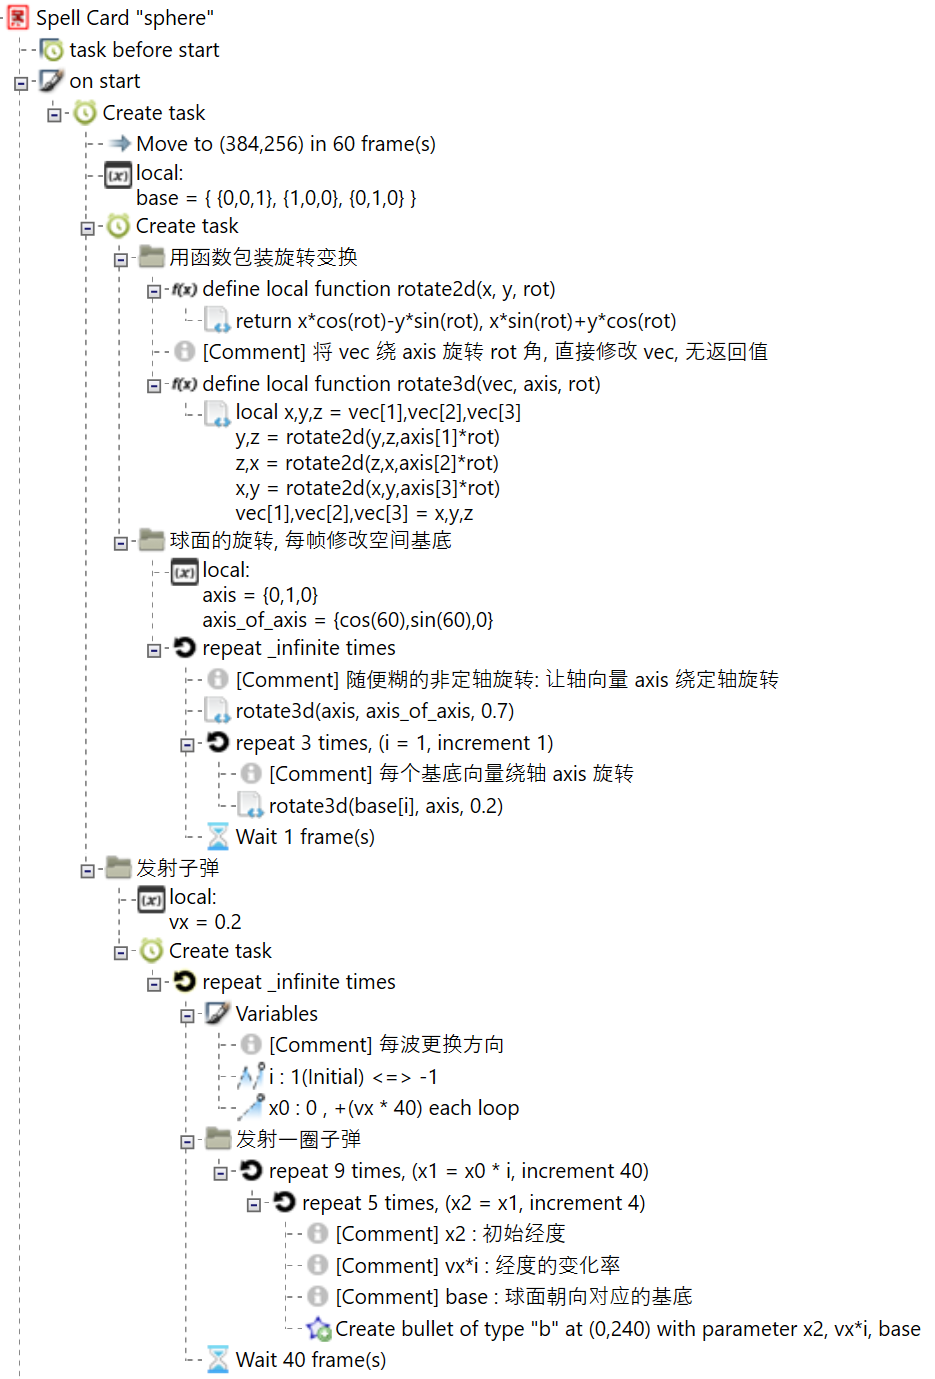
\includegraphics[width=0.54\textwidth]
  {assets/3d/eg1-4.png}
  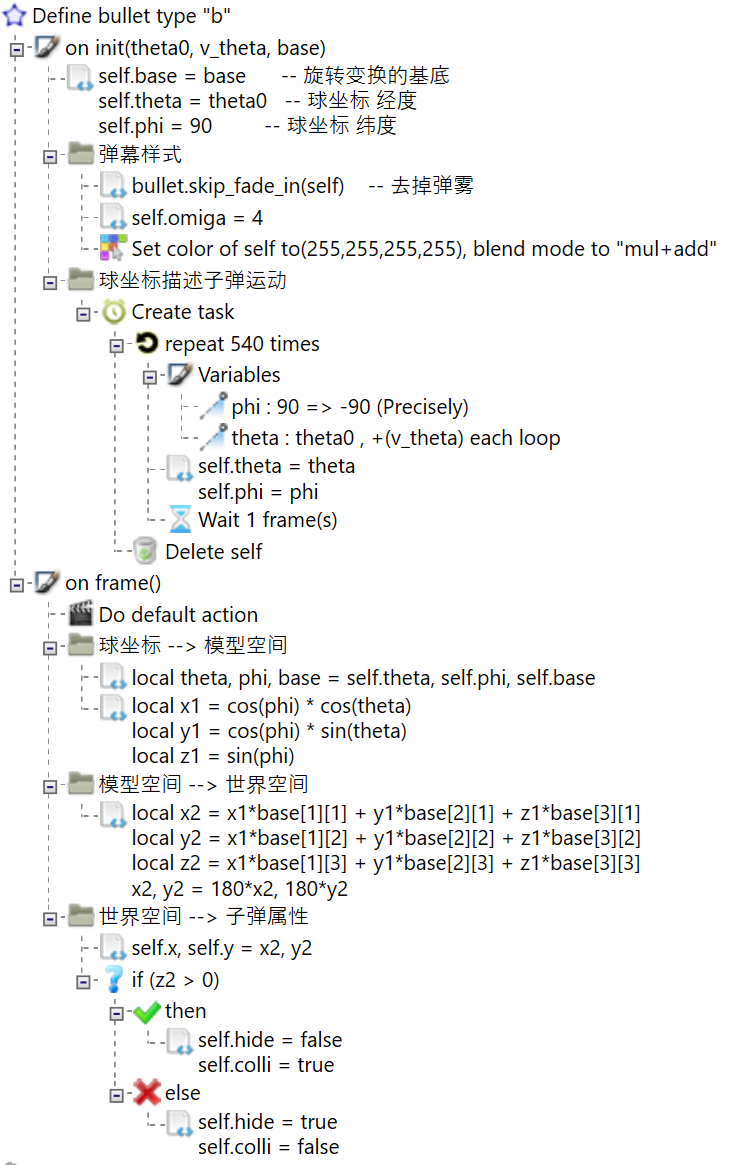
\includegraphics[width=0.44\textwidth]
  {assets/3d/eg1-5.png}
  \caption{伪3D弹幕工程}
  \label{fig:3d-spellcard-code}
\end{figure}

\subsection{例2: 3D背景}

这个例子中我们讨论3D背景中的三维坐标与屏幕上的二维坐标是怎么对应的,
主要涉及视图变换的后三步: 摄像机变换, 投影变换和视口变换.
以LuaSTG自带的cube\_background为例.

在背景的lua脚本中, 我们在三维场景中渲染一些图片来搭建场景
(使用Render4V函数, 指定图片的四个顶点在场景中的三维坐标来完成一次渲染).
如图\ref{subfig:cube-world},
对于左边的两列立方体, 我们渲染它们的右,上,前三个面;
右边的两列立方体则渲染左,上,前三个面,
每个面使用如下的图片素材.
图片的渲染位置一般是容易确定的, 不涉及三维旋转等复杂计算.

\begin{center}
  
\includegraphics[width=2cm]
  {assets/3d/cube-face.png}
\end{center}

lua脚本中还会设置一些参数, 如下面的代码所示,
参数包括eye, at, up, z, fovy, fog.
一会我们会说到这些参数都是干什么的.
我们编写背景的lua脚本时不需要去计算视图变换,
视图变换由LuaSTG的引擎自动完成 (基于DirectX).

\begin{lstlisting}
Set3D("eye", 0, 3.3, -3.8)
Set3D("at", 0, 1.5, -0.4)
Set3D("up", -1.8, 1, 0)
Set3D("z", 1, 100)
Set3D("fovy", 0.6)
Set3D("fog", 3, 10, Color(0xFF1E46FF))
\end{lstlisting}

\begin{figure}[htbp]
  \centering
  \begin{subfigure}{0.24\textwidth}
    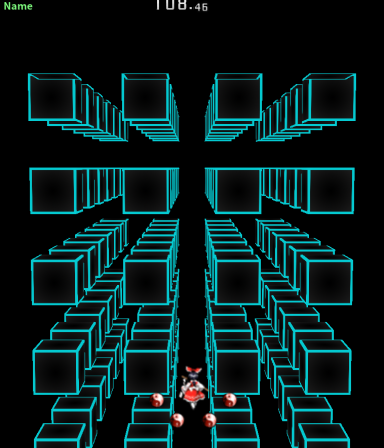
\includegraphics[width=\textwidth]
    {assets/3d/eg2-1.png}
    \caption{场景 (世界空间)}
    \label{subfig:cube-world}
  \end{subfigure}
  \begin{subfigure}{0.24\textwidth}
    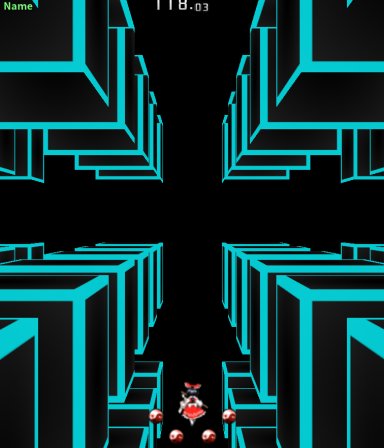
\includegraphics[width=\textwidth]
    {assets/3d/eg2-2.png}
    \caption{设置摄像机位置}
    \label{subfig:cube-camera-eye}
  \end{subfigure}
  \begin{subfigure}{0.24\textwidth}
    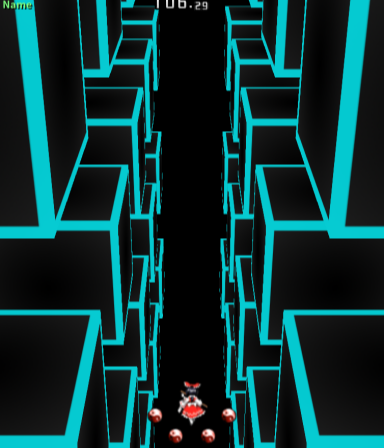
\includegraphics[width=\textwidth]
    {assets/3d/eg2-3.png}
    \caption{设置摄像机观察方向}
    \label{subfig:cube-camera-at}
  \end{subfigure}
  \begin{subfigure}{0.24\textwidth}
    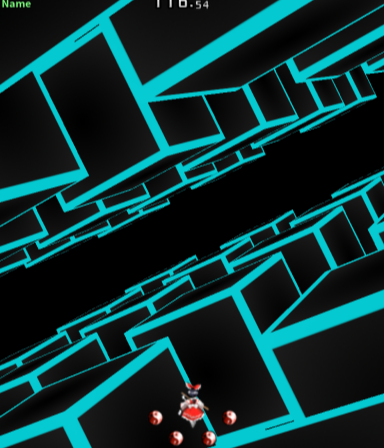
\includegraphics[width=\textwidth]
    {assets/3d/eg2-4.png}
    \caption{设置摄像机正上方向}
    \label{subfig:cube-camera-up}
  \end{subfigure}
  \caption{cube\_background}
\end{figure}

\subsubsection{摄像机变换: 世界空间$\to$摄像机空间}

\def\eye{\vv{\text{eye}}}
\def\at{\vv{\text{at}}}
\def\up{\vv{\text{up}}}

第一步, 引擎要根据我们设置的参数, 在场景中设置一个摄像机,
把场景中的坐标转换成相对于摄像机的坐标, 这就是摄像机变换.
这一步需要用到的参数为eye, at和up, 对应着三个坐标,
我们用$\eye,\at,\up$三个向量来表示.

首先要说明的是, 在3D背景中, 我们使用的是\emph{左手坐标系},
默认的坐标轴朝向为: $x$轴向右, $y$轴向上, $z$轴垂直于屏幕向里.
图\ref{subfig:cube-world}就是用这个默认的坐标轴朝向展示的场景.
如果你正在用顺时针/逆时针描述三维空间的旋转方向,
一定要注意你所想的逆时针方向是对应
$x\to y\to z\to x\to\cdots$
还是$z\to y\to x\to z\to\cdots$,
不然在计算旋转时容易出现错误.

说回摄像机的参数, $\eye$是摄像机在场景中的位置,
如图\ref{subfig:cube-camera-eye},
通过设置$\eye$我们可以把摄像机放到场景中这些立方体之间;
$\at$是摄像机看向的一个位置,
如图\ref{subfig:cube-camera-at},
设置$\at$让摄像机机向下看 (掩盖我们没有渲染立方体底面的骗局bushi).
$\up$是指示摄像机向上方向的一个向量,
如图\ref{subfig:cube-camera-up},
设置$\up$让摄像机倾斜着观察场景.

\begin{center}
  \begin{tikzpicture}[scale=0.5]
    \draw[-latex] (-5,0) -- (5,0) node[right] {$z$};
    \draw[-latex] (0,-1) -- (0,5) node[left] {$y$};
    \draw[-latex] (-3.8,3.3)
    node[above] {eye $(0,3.3,-3.8)$} node[dot] {}
    -- (-0.4,1.5)
    node[below,background] {at $(0,1.5,-0.4)$} node[dot] {};

    \draw[-latex,dashed] (0,0,0) -- (0,0,5) node[left] {$x$};
  \end{tikzpicture}
\end{center}

我们以摄像机位置eye为原点建立直角坐标系,
使得在摄像机的视角下, $x$轴向右, $y$轴向上, $z$轴垂直于屏幕向里.
为了把场景中的坐标转换到摄像机空间,
我们需要计算摄像机空间对应的标准正交基
$(\vec e_1,\vec e_2,\vec e_3)$.
标准正交基的概念见\ref{sec:vector-base}节.

$\vec e_1,\vec e_2,\vec e_3$分别对应摄像机空间的$x,y,z$轴.
$\vec e_3$垂直于屏幕向里, 与eye指向at的方向一致,
所以我们把$(\at-\eye)$单位化 (放缩为单位向量), 就得到了$\vec e_3$.
\[
  \vec e_3 = \dfrac{\at-\eye}{|\at-\eye|}.
\]

如下图所示, $\up$的方向实际上可以不是严格的竖直朝上,
所以不能把$\up$直接放缩为单位向量来得到$\vec e_2$.

\begin{center}
  \begin{tikzpicture}
    \draw[help lines] (0,0) node[dot,label={left:eye}] {}
    -- (2,0) node[dot,label={right:at}] {};
    \draw[-latex,gray] (0,0) -- (1,1.5) node[right] {$\up$};
    \draw[help lines,dashed] (1,0) -- (1,1.5) -- (0,1.5) -- (0,1);

    \draw[-latex] (0,0) -- (1,0) node[below] {$\vec e_3$};
    \draw[-latex] (0,0) -- (0,1) node[left] {$\vec e_2$};
    \draw[-latex] (0,0) -- (0,0,1) node[below] {$\vec e_1$};
  \end{tikzpicture}
\end{center}

我们可以先计算$\vec e_1$.
$\vec e_1$垂直于$\up$和$\vec e_3$所在的平面,
这与三维向量外积的几何含义一致,
可以用三维向量的外积来计算它的方向.
考虑到$\vec e_1,\up,\vec e_3$构成左手系,
我们计算$\up\times\vec e_3$, 它的方向与$\vec e_1$方向相同,
把它单位化就得到$\vec e_1$.
\[
  \vec e_1 = \dfrac{\up\times\vec e_3}{|\up\times\vec e_3|}.
\]

有了$\vec e_1$和$\vec e_3$, 我们可以直接计算$\vec e_2$:
\[
  \vec e_2 = \vec e_3\times\vec e_1.
\]

设有一个点在场景中的坐标为$\vec P$, 在摄像机空间的坐标为$(x,y,z)$.
根据空间基底的概念, 我们知道
$\vec P = \eye + x\vec e_1 + y\vec e_2 + z\vec e_3$.
利用标准正交基的性质, 我们可以用内积计算$x,y,z$:
\begin{align*}
  x = (\vec P - \eye)\cdot\vec e_1, \\
  y = (\vec P - \eye)\cdot\vec e_2, \\
  z = (\vec P - \eye)\cdot\vec e_3.
\end{align*}

\subsubsection{投影变换 (简化): 摄像机空间$\to$标准平面}

第二步, 引擎要把摄像机空间的坐标投影到一个平面上,
使得摄像机能够看见的区域被投影到
$-1\le x\le1,-1\le y\le1$的矩形区域, 该区域被称为\emph{标准视体}.
这个平面就被称为标准平面.
根据摄像机可见区域的形状, 引擎会使用正交投影或者透视投影.

正交投影, 又称平行投影, 对应的可视区域是一个简单的长方体.
如下图所示, 摄像机的可视区域为
$
  \text{left} \le x \le \text{right},
  \text{bottom} \le y \le \text{top},
  \text{near} \le z \le \text{far}.
$

\begin{center}
  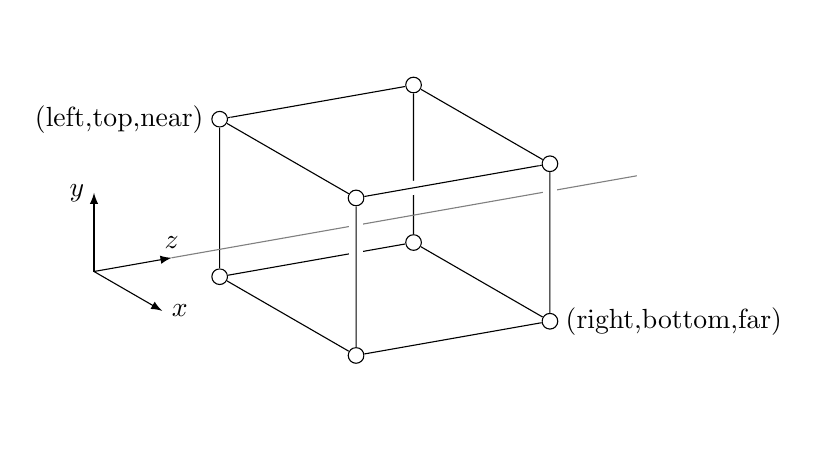
\begin{tikzpicture}[
      x=(-30:1cm),
      y=(90:1cm),
      z=(10:1cm),
      declare function = {
          l = -1;   r = 1;
          b = -1;   t = 1;
          n = 2.5;  f = 5;
        }
    ]
    \draw[-latex] (0,0,0) -- (1,0,0) node[right] {$x$};
    \draw[-latex] (0,0,0) -- (0,1,0) node[left] {$y$};
    \draw[-latex] (0,0,0) -- (0,0,1) node[above] {$z$};

    \begin{scope}[circle,inner sep=2pt]
      \node[draw,label={left:(left,top,near)}]
      (a) at (l,t,n) {};
      \node[draw] (b) at (l,t,f) {};
      \node[draw] (c) at (r,t,f) {};
      \node[draw] (d) at (r,t,n) {};
      \node[draw] (e) at (l,b,n) {};
      \node[draw] (f) at (l,b,f) {};
      \node[draw,label={right:(right,bottom,far)}]
      (g) at (r,b,f) {};
      \node[draw] (h) at (r,b,n) {};
    \end{scope}

    \draw[preaction={draw,white,line width=5pt}]
    (e) -- (f) -- (g) -- (h) -- (e);
    \draw[preaction={draw,white,line width=5pt}]
    (e) -- (a) -- (b) -- (f);
    \draw[gray] (0,0,1) -- (0,0,7);
    \draw[preaction={draw,white,line width=5pt}]
    (h) -- (d) -- (c) -- (g);
    \draw[preaction={draw,white,line width=5pt}]
    (a) -- (d) (b) -- (c);
  \end{tikzpicture}
\end{center}

我们暂时不考虑对$z$坐标的处理, 这涉及到遮挡和裁剪等比较复杂的话题.
只考虑如何计算投影后的$(x,y)$坐标.
对于正交投影, 显然$z$坐标与投影结果无关,
我们只需要考虑$x,y$所在的矩形发生怎样的变化.
如下图, 将可视区域的矩形经过简单的平移和缩放, 就可以得到标准视体.

\begin{center}
  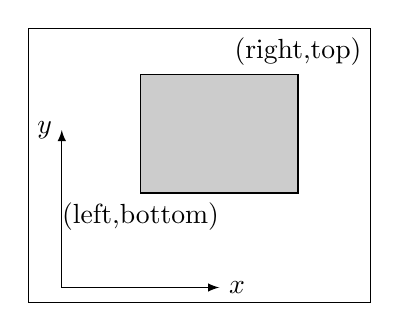
\begin{tikzpicture}[baseline=(current bounding box.center)]
    \draw[-latex] (0,0) -- (2,0) node[right] {$x$};
    \draw[-latex] (0,0) -- (0,2) node[left] {$y$};
    \draw[fill=gray,fill opacity=0.4]
    (1,1.2) coordinate (a)
    rectangle (3,2.7) coordinate (b);
    \node[below] at (a) {(left,bottom)};
    \node[above] at (b) {(right,top)};
    \draw (current bounding box.south west)
    rectangle (current bounding box.north east);
  \end{tikzpicture}
  $\quad\implies\quad$
  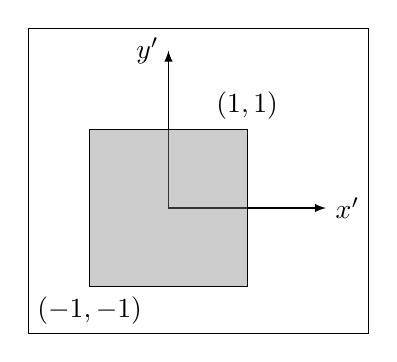
\begin{tikzpicture}[baseline=(current bounding box.center)]
    \draw[-latex] (0,0) -- (2,0) node[right] {$x'$};
    \draw[-latex] (0,0) -- (0,2) node[left] {$y'$};
    \draw[fill=gray,fill opacity=0.4]
    (-1,-1) coordinate (a)
    rectangle (1,1) coordinate (b);
    \node[below] at (a) {$(-1,-1)$};
    \node[above] at (b) {$(1,1)$};
    \draw (current bounding box.south west)
    rectangle (current bounding box.north east);
  \end{tikzpicture}
\end{center}

\begin{align*}
  x' & =
  \left(x - \dfrac{\text{left}+\text{right}}{2}\right)
  \cdot\dfrac{2}{\text{right}-\text{left}}, \\
  y' & =
  \left(y - \dfrac{\text{bottom}+\text{top}}{2}\right)
  \cdot\dfrac{2}{\text{top}-\text{bottom}}.
\end{align*}

透视投影模拟人眼看东西的原理, 遵循近大远小的原则.
透视投影所对应的可视区域是一个锥体, 如下图所示, 这个锥体被称为视锥.

\begin{center}
  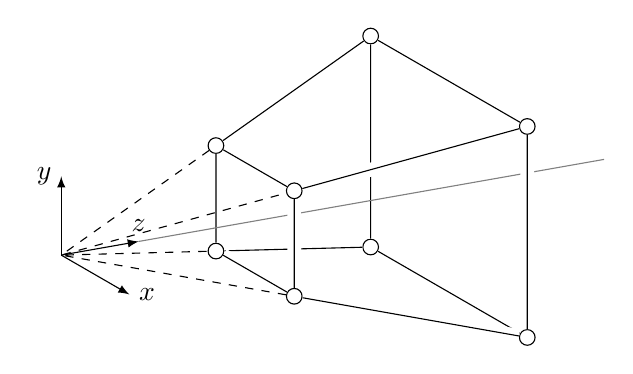
\begin{tikzpicture}[
      x=(-30:1cm),
      y=(90:1cm),
      z=(10:1cm),
      declare function = {
          t = 30; a = 192/224;
          n = 2.5; f = 5;
        }
    ]
    \draw[-latex] (0,0,0) -- (1,0,0) node[right] {$x$};
    \draw[-latex] (0,0,0) -- (0,1,0) node[left] {$y$};
    \draw[-latex] (0,0,0) -- (0,0,1) node[above] {$z$};

    \begin{scope}[circle,inner sep=2pt]
      \coordinate (0) at (0,0);
      \node[draw] (1) at ({-a*n*tan(t/2)},{n*tan(t/2)},n) {};
      \node[draw] (2) at ({a*n*tan(t/2)},{n*tan(t/2)},n) {};
      \node[draw] (3) at ({a*n*tan(t/2)},{-n*tan(t/2)},n) {};
      \node[draw] (4) at ({-a*n*tan(t/2)},{-n*tan(t/2)},n) {};
      \node[draw] (5) at ({-a*f*tan(t/2)},{f*tan(t/2)},f) {};
      \node[draw] (6) at ({a*f*tan(t/2)},{f*tan(t/2)},f) {};
      \node[draw] (7) at ({a*f*tan(t/2)},{-f*tan(t/2)},f) {};
      \node[draw] (8) at ({-a*f*tan(t/2)},{-f*tan(t/2)},f) {};
    \end{scope}

    \draw[preaction={draw,white,line width=5pt}]
    (1) -- (5) -- (8) -- (4) -- (1);
    \draw[gray] (0,0,1) -- (0,0,7);
    \draw[preaction={draw,white,line width=5pt}]
    (1) -- (2) -- (3) -- (4);
    \draw[preaction={draw,white,line width=5pt}]
    (5) -- (6) -- (7) -- (8);
    \draw[preaction={draw,white,line width=5pt}]
    (2) -- (6) (3) -- (7);

    \draw[dashed] (1) -- (0) -- (2) (3) -- (0) -- (4);
  \end{tikzpicture}
\end{center}

3D背景使用的正是透视投影, 背景的参数fovy和z对应着透视投影的参数.

fovy是``\textcolor{red}{f}ield \textcolor{red}{o}f
\textcolor{red}{v}iew \textcolor{red}{$y$}''的缩写,
field of view就是视野的意思.
如下图, fovy是一个角, 表示在$y$方向的视野范围,
需要注意在实际应用中它的大小用弧度制表示.

背景的参数z对应下图的near和far两个数值,
与前面的正交投影一样, 我们暂且不考虑near和far的事情.

透视投影还有一个参数aspect ratio, 对应中文是宽高比,
表示视锥的宽度和高度的比例.
在LuaSTG中, 这个宽高比就是游戏版面的宽高比$192/224$.

\begin{center}
  \begin{tikzpicture}[
      declare function = {
          t = 30; a = 192/224;
          n = 2.5; f = 5;
        }
    ]
    \draw[-latex] (1,0) -- (7,0) node[right] {$z$};
    \draw[-latex] (0,-1) -- (0,1) node[left] {$y$};
    \node[left] {$O$};

    \coordinate (1) at (n,{n*tan(t/2)});
    \coordinate (2) at (f,{f*tan(t/2)});
    \coordinate (3) at (f,{-f*tan(t/2)});
    \coordinate (4) at (n,{-n*tan(t/2)});

    \draw[help lines] (1) -- (0,0) -- (4);
    \draw ({-t/2}:4mm) arc ({-t/2}:{t/2}:4mm)
    node[midway,background,right] {fovy};
    \draw[fill=gray,fill opacity=0.4]
    (1) -- (2) -- (3) -- (4) -- cycle;
    \node[below right] at (n,0) {$z=\text{near}$};
    \node[below right] at (f,0) {$z=\text{far}$};
  \end{tikzpicture}
\end{center}

在透视投影中, 一条经过原点的直线上的所有点将对应标准平面上的同一点.
对于空间中的点$(x,y,z)$, 它投影到标准平面的点$(x',y')$,
那么$x',y'$将会与$x/z,y/z$呈正比.

考虑视锥的边界线, 边界线上的$x/z$和$y/z$应当投影到标准平面的$1$.
设$\theta = \text{fovy}, a = \text{aspect ratio}$, 那么边界线上有
\[
  y/z = \tan(\theta/2),\quad
  x/z = x/y \cdot y/z = a\tan(\theta/2).
\]

这样我们就知道标准平面的$x',y'$与空间中$x/z,y/z$的比例关系.
对于摄像机空间的点$(x,y,z)$, 投影到标准平面上的坐标为
\[
  x' = \dfrac{x}{z}\cdot\dfrac{1}{a\tan(\theta/2)},\quad
  y' = \dfrac{y}{z}\cdot\dfrac{1}{\tan(\theta/2)}.
\]

\subsubsection{视口变换}

第三步, 引擎要把标准视体内的坐标变换到屏幕分辨率范围内,
这一步比较简单, 不过涉及到一个我们很不常用的屏幕坐标系,
篇幅原因这里就不作介绍了.

不过我们可以很容易地把标准视体内的坐标变换到游戏版面范围,
也就是$-192\le x'\le192, -224\le y'\le224$:
\[
x' = 192x,\quad y' = 224y.
\]

\subsubsection{投影变换的补充}

前面我们说投影变换是从三维的摄像机空间投影到二维的标准平面,
这是为了更简单地完成讲解. 实际上投影变换得到的是一个三维的标准空间,
标准视体除了$-1\le x\le1, -1\le y\le1$之外,
还会把摄像机可视范围的$\text{near}\le z\le\text{far}$
变换到$0\le z\le1$. 这是为了进行裁剪,
裁剪会把标准视体之外的内容丢弃掉.
毕竟我们不太希望GPU去计算摄像机身后或者离摄像机太远的内容,
裁剪掉它们可以节省大量的计算资源.

对于正交投影, 由于LuaSTG的正交投影一般只用在2D场景,
比如制作弹幕/UI的场景,
所以正交投影摄像机的可视范围总是$0\le z\le1$,
计算正交投影时$z$坐标保持不变即可.
我们在2D场景使用Render4V函数时,
顶点的$z$坐标按照惯例都填0.5, 就是因为它是0到1之间的一个数.
如果超出0到1的范围, 引擎会进行裁剪使得渲染内容与我们的预期不同.

对于透视投影, near和far需要我们自己指定
(在制作3D背景时). 由于透视投影需要除以$z$坐标,
我们在指定near和far时需要满足
$0 < \text{near} < \text{far}$.
另外有一个很有意思的事情: 一条直线经过透视投影之后仍然是直线.

虽然我很想聊一聊更贴近真实计算方式的透视投影,
也就是通过百度能找到的基于齐次坐标的透视投影计算,
通过齐次坐标我们能更好地理解透视投影的本质.
但是这样讲有些太累了, 我的表达能力还不足以让我把它讲明白,
最后只能徒增学习难度罢了.

那么这一节的内容就到这里,
不出意外的话这也是本教程的最后一节.
感谢读者你能看到这里, 我真心希望我写的这些东西能给你带来一点收获.

